\documentclass[conference]{IEEEtran}

\pagestyle{plain}

\usepackage[utf8]{inputenc}
\usepackage{graphicx}
\usepackage{xcolor}
\usepackage{svg}
\usepackage{booktabs}
\usepackage{multirow}
\usepackage{amsmath}
\usepackage{algpseudocode}
\usepackage{listings}
\usepackage{subcaption}
\usepackage{comment}
\usepackage[hidelinks]{hyperref}
%\usepackage[T1]{fontenc}
%\usepackage{lmodern} % TODO: work out why this doesn't compile without this https://tex.stackexchange.com/questions/10706/pdftex-error-font-expansion-auto-expansion-is-only-possible-with-scalable
\lstset{
  basicstyle=\ttfamily,
  columns=fullflexible,
  frame=single,
  breaklines=true,
  tabsize=4,
}

\begin{document}

\title{Dishy Paper}
% Dishing out Disaster
% Dishing out DoS
% The Dishy Terminator
% Space Oddity
% Fuzzing with the Stars
% Starlink: Dish Served Cold

\author{Anonymous Authors}

\begin{comment}
\author{\IEEEauthorblockN{Joshua Smailes}
\IEEEauthorblockA{University of Oxford\\
joshua.smailes@cs.ox.ac.uk}
\and
\IEEEauthorblockN{Edd Salkield}
\IEEEauthorblockA{University of Oxford\\
edd.salkield@cs.ox.ac.uk}
\and
\IEEEauthorblockN{Simon Birnbach}
\IEEEauthorblockA{University of Oxford\\
simon.birnbach@cs.ox.ac.uk}
\and
\IEEEauthorblockN{Martin Strohmeier}
\IEEEauthorblockA{Cyber-Defence Campus, armasuisse Science + Technology\\
martin.strohmeier@armasuisse.ch}
\and
\IEEEauthorblockN{Ivan Martinovic}
\IEEEauthorblockA{University of Oxford\\
ivan.martinovic@cs.ox.ac.uk}}
\end{comment}

\IEEEoverridecommandlockouts
\makeatletter\def\@IEEEpubidpullup{6.5\baselineskip}\makeatother
\IEEEpubid{\parbox{\columnwidth}{
    Network and Distributed System Security (NDSS) Symposium 2023\\
    28 February - 4 March 2023, San Diego, CA, USA\\
    ISBN 1-891562-83-5\\
    https://dx.doi.org/10.14722/ndss.2023.23xxx\\
    www.ndss-symposium.org
}
\hspace{\columnsep}\makebox[\columnwidth]{}}

\maketitle

\begin{abstract}
The Starlink user terminal is vulnerable to a denial-of-service attack, in which the dish is put into an inoperative state until it can be manually rebooted by physically power-cycling the terminal.

In this paper we describe this attack in detail, including the fuzzing process used to discover it.
We also explore the impact of the attack, particularly in the cases of drive-by attackers, and attackers that are able to maintain a continuous presence on the network.
Finally, we discuss the wider implications, looking at common security challenges faced by commercial routers, and how they can be mitigated without sacrificing user experience.
\end{abstract}

\section{Motivation}\label{sec:motivation}

The Starlink user terminal, similarly to other consumer routers, is configured through a web admin page accessible on the local network.
This page makes API calls over the local network to query and update the state, therefore providing a promising attack surface for adversaries to attempt to configure the state or deny service by injecting malformed commands.

It is well known that other routers are vulnerable to these techniques.
Since traffic on the local network is seldom encrypted, local attackers can scrape admin passwords and potentially inject commands.
Additionally, default admin passwords, combined with browser policies typically allowing cross-origin writes~\cite{same_origin_policy,csrf_internal_network}, have also resulted in configurations vulnerable to attack from outside the local network~\cite{drive_by_pharming}.

However, unlike other consumer routers, these commands are not password authenticated.
This allows any device on the local network to send commands to the user terminal, and therefore exploit any vulnerabilities in the command decoding and execution logic.
This also allows allows insecure devices and certain network configurations to be leveraged by external attackers to inject commands from outside the network.
Additionally, the lack of rate limiting allows potential adversaries to scan the user terminal for potential vulnerabilities by fuzzing.

In this work we therefore present a security analysis of the Starlink user terminal administrative interface.
In Section~\ref{sec:attack}, we present a novel attack in which a malformed command can be sent to put the user terminal into an inoperative state until it can be physically power-cycled.
In Section~\ref{sec:impact}, we consider the impact of this attack in different scenarios where the configuration command interface can be exploited by on-network adversaries.
In Section~\ref{sec:discussion}, we discuss the security properties of the system overall, including against remote adversaries who may use browser exploits, IP spoofing, and DNS hijacking to send commands.

\section{Attack}\label{sec:attack}

\begin{figure*}
    \centering
    \begin{subfigure}{.15\textwidth}
        \centering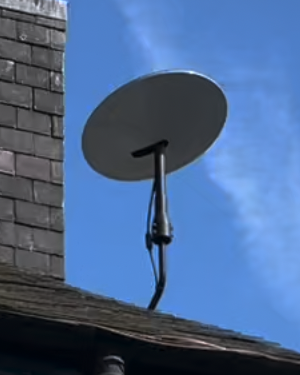
\includegraphics[width=\textwidth]{img/unstowed.png}\\\vspace{.35em}
        \centering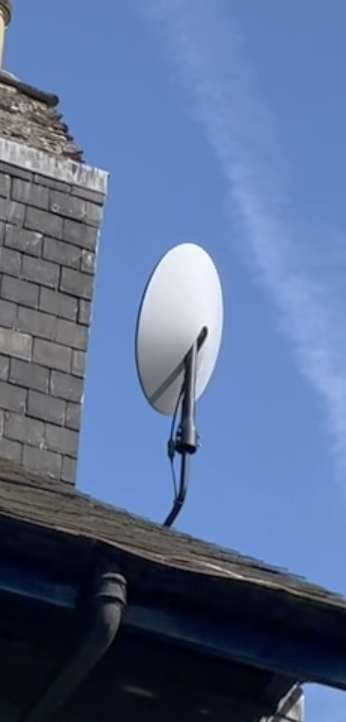
\includegraphics[width=\textwidth]{img/stowed.png}
        \caption{The dish in ``active'' and ``stowed'' modes.}
    \end{subfigure}
    \hspace{0.00005\textwidth}
    \begin{subfigure}{.4335\textwidth}
        \centering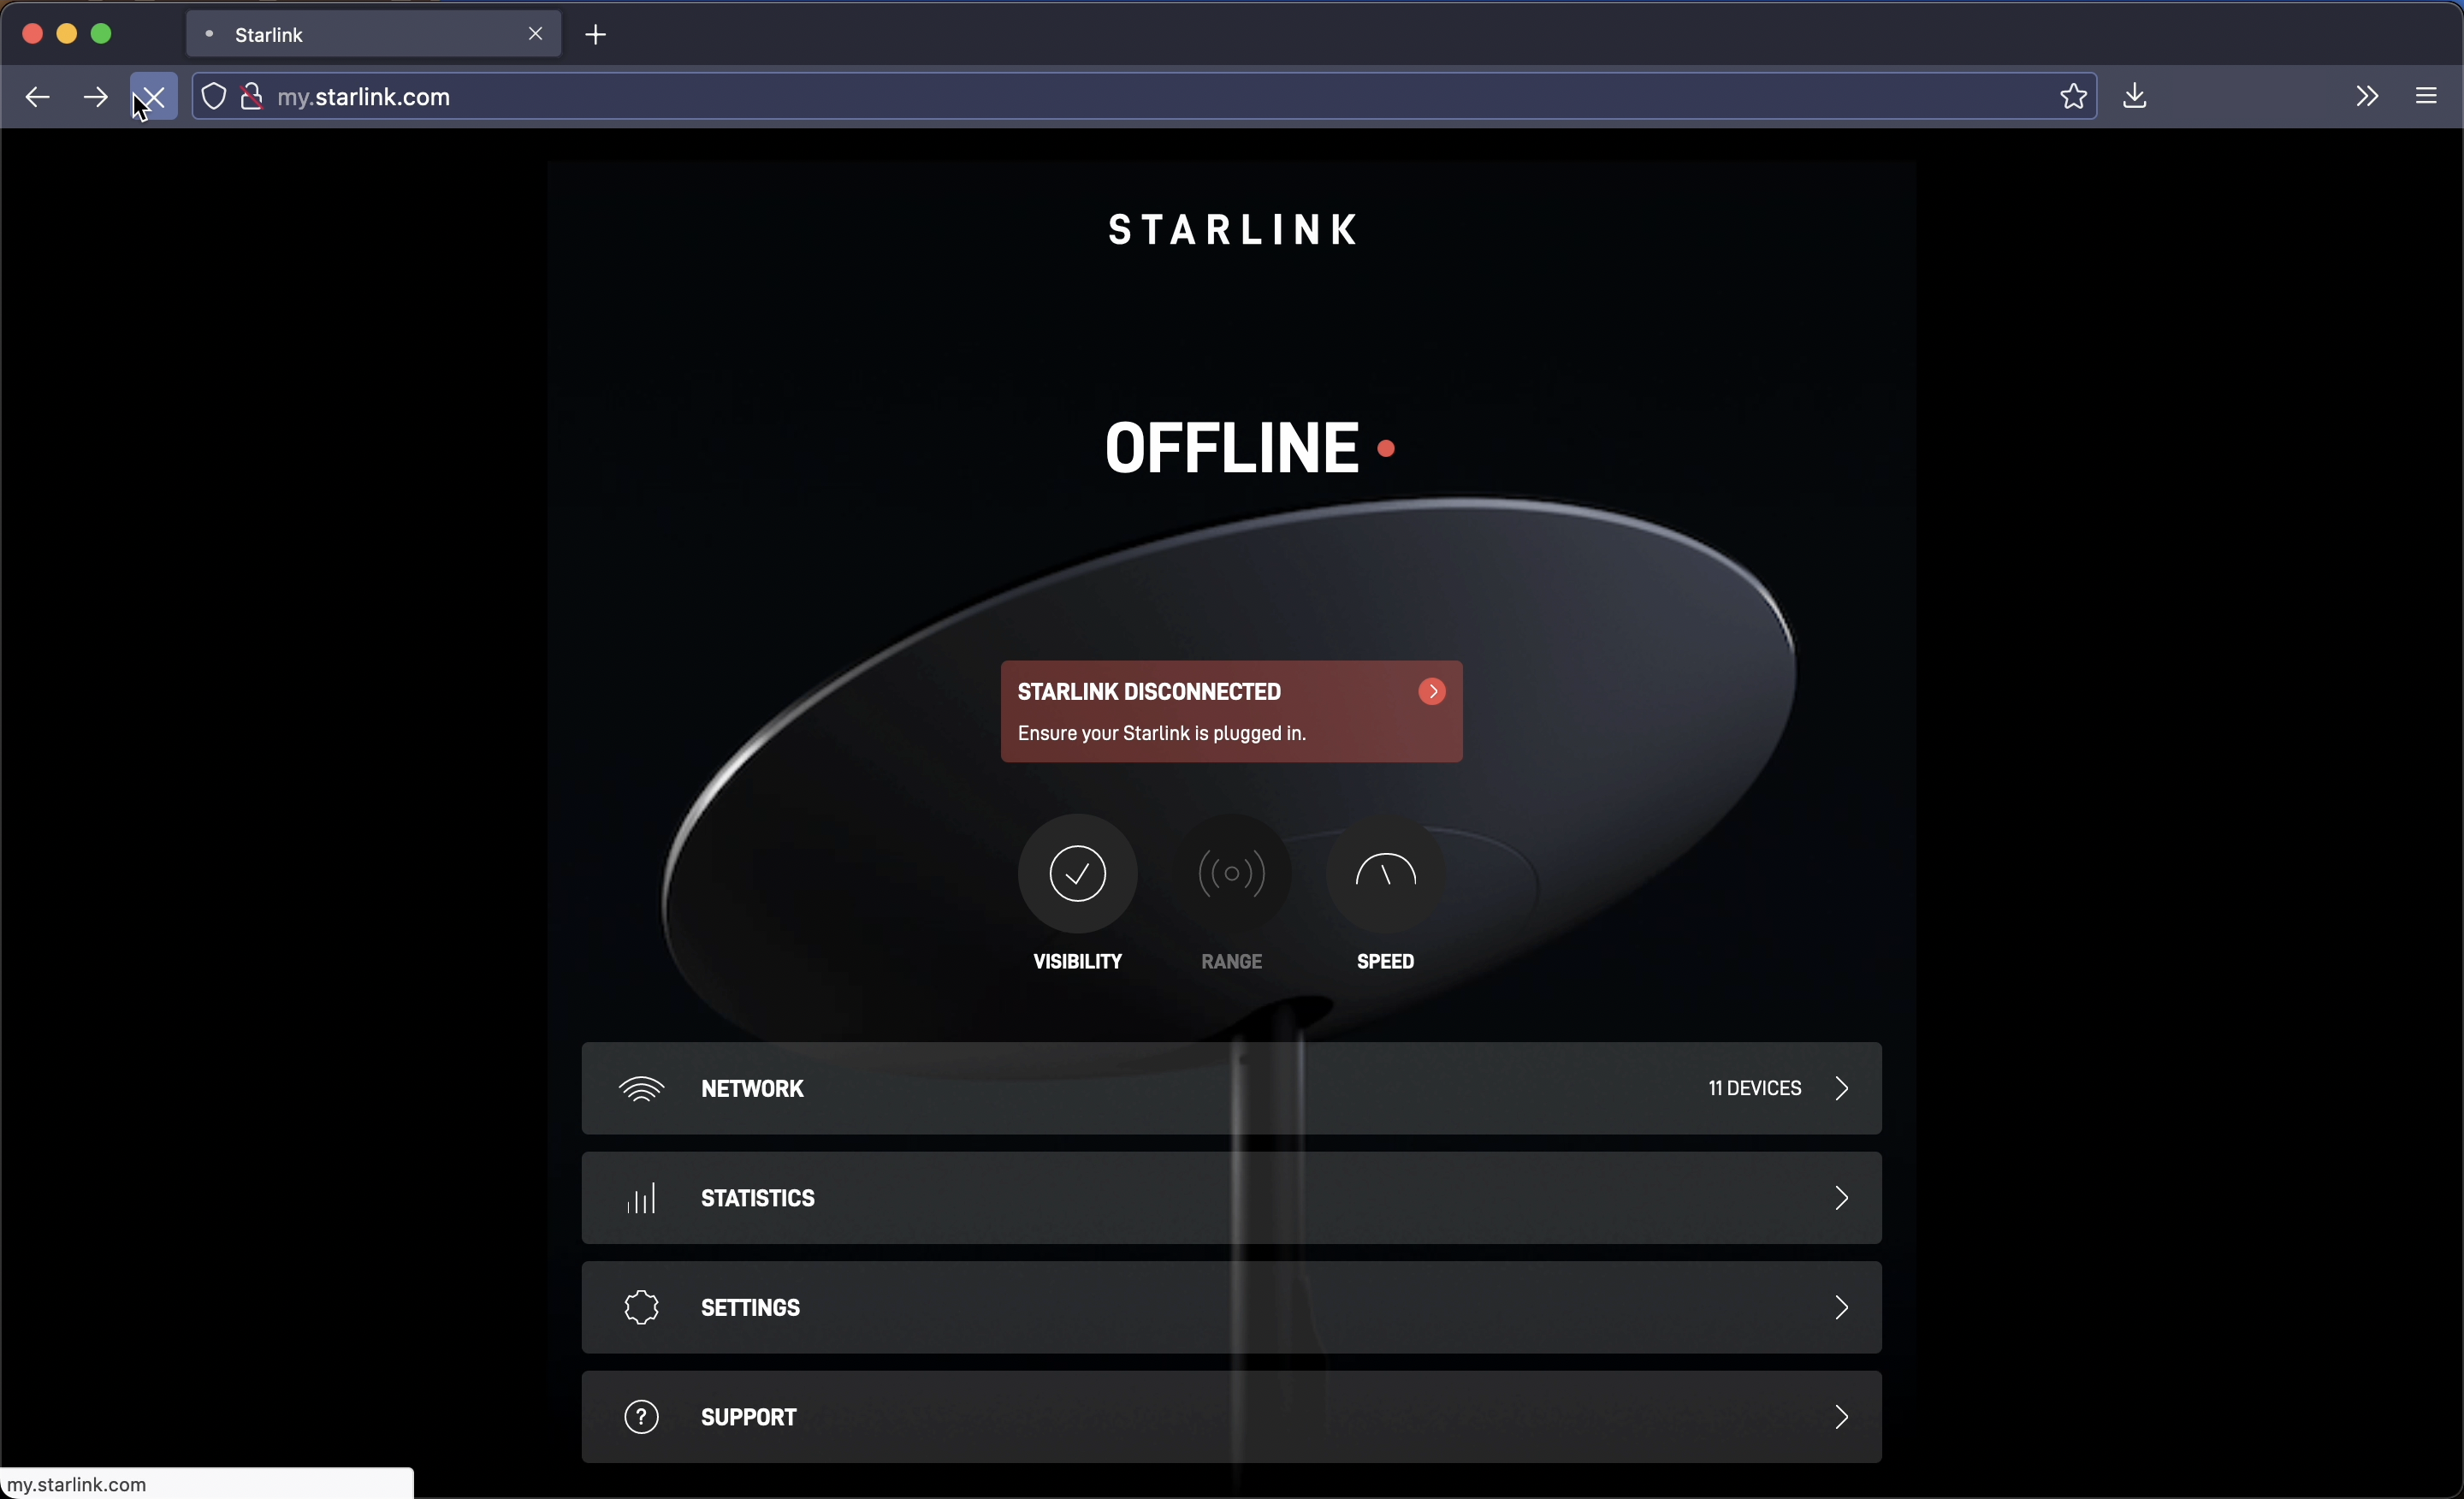
\includegraphics[width=\textwidth]{img/offline.png}\\\vspace{.35em}
        \centering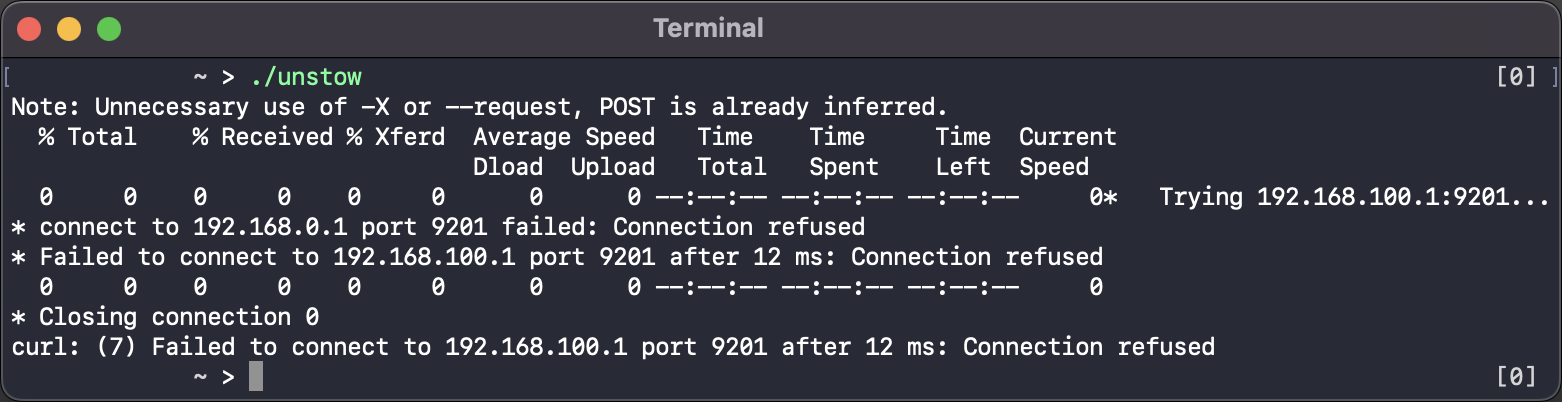
\includegraphics[width=\textwidth]{img/unstow.png}
        \caption{The web control panel error screen following the attack, and the result of sending commands to an inoperative dish\footnotemark[1].}
    \end{subfigure}
\vspace{-0.7em}
\caption{The outcome of a successful attack on the Starlink dish, and the resulting web control panel and response to commands.}
\label{fig:attack-outcome}
\vspace{-1.5em}
\end{figure*}

The Starlink user terminal is typically administered via the ``\url{http://my.starlink.com}'' web interface, which sends gRPC commands to the modem over the local network.
As shown in Figure~\ref{fig:modem}, these requests are decoded by a gRPC web proxy and forwarded to a command handler.

The vast majority of gRPC commands require no authentication, including commands affecting the physical state of the dish.
We note, in particular, that the ``dish stow'' command, which stops communication with the satellites, requires no authentication.

Since the gRPC payload is usually between 2 and 5 bytes, the command space can be fuzzed with random contents to discover unexpected behavior in the command handler\footnote{Source code available at \textit{\url{https://github.com/ssloxford/dishing-out-dos}}}.
Through this we discovered invalid command \lstinline{00 00 00 00 03 EA 3E 00} which causes the command handler of the user terminal to crash and no longer respond to commands.
This allows the attacker to lock the physical dish into a stowed state as seen in Figure~\ref{fig:attack-outcome}, persistently denying service even after the attacker is no longer present on the network.
Restoring internet access requires a physical power-cycle.

\section{Impact}\label{sec:impact}

This attack can have a signficant impact -- since the state of the dish is frozen, an adversary can achieve persistent denial of service by first sending a command to stow the dish.
This will interrupt service until the dish can be physically power-cycled, which is not always trivial.
As long as the adversary remains on the local network, this attack can be repeated to cause continuous loss of service for users on the network.
Therefore, attackers that can maintain presence on the network will have the greatest impact.

There is also potential for remote attacks, provided the attacker can in some way cause a device on the same network as the dish to send HTTP requests.
The Cross-Origin Resource Sharing (CORS) \textbf{TODO cite} policies of modern browsers prevent javascript from making unauthorized requests to external domains or addresses, so javascript-based attacks are unlikely unless legacy browsers are used.
However, the attacker could trick a user into executing a malicious executable or script, which could easily be used to make these requests.

Furthermore, in some cases ``drive-by'' attacks are possible -- if the network is not password protected, an attacker can connect and execute the attack while passing nearby.
Since the Starlink routers do not have passwords by default, this could be a serious concern.
Executing the attack only requires a few seconds of connection on the local network, and can cause outages on the order of minutes or hours.
This can be mitigated by using the ``guest network'' mode provided by the router -- this adds an unprotected guest network which does not have access to the administrative interface.

Since the attack can be deployed from any device connected to the local network, large networks containing many untrusted users are at the greatest risk.
Such networks also suffer greater impact, as more devices are affected by network disruptions.
The impact is magnified when Starlink is the only source of internet access for that customer.
Examples may include maritime and aviation traffic, internet cafés, or large organisations.

Restoring service requires physical access to the terminal, so disruption will be increased where access is difficult or restricted.
Examples may include secured rooftop installations.

\subsection{Responsible Disclosure}\label{sec:responsible-disclosure}

This vulnerability has been reported to Starlink through their provided channels.
It has been triaged and reproduced by their security team, and the root cause was determined to be a bug in the gRPC server's handling of edge cases.
A fix for this problem will have been fully deployed by the time of this paper's publication.

\section{Discussion}\label{sec:discussion}

Yes

\begin{comment}
  Edd's notes:

Related work:

Zoom exploit, hitting services running on the local network

https://developer.mozilla.org/en-US/docs/Web/Security/Same-origin_policy
"Cross-origin writes are typically allowed"

https://bugzilla.mozilla.org/show_bug.cgi?id=629094
https://www.grepular.com/Abusing_HTTP_Status_Codes_to_Expose_Private_Information
HTTP status code abuse to extract information cross-origin

https://bugzilla.mozilla.org/show_bug.cgi?id=354493
Zoom videoconferencing problem

https://bugzilla.mozilla.org/show_bug.cgi?id=371598
Drive-by pharming through browsers


Security constraints:

Defeating drive-by javascript:
unencrypted passwords prevents silent drive-by javascript, potentially
websites can still brute force or phish the password from you
some sort of CSRF token from my.starlink.com?

Defeating spoofing my.starlink.com:
Vulnerable: because it's using plaintext http
Reason: you can't make a request to an insecure origin from a secure origin (need citation)
use https
passwords prevent silently changing the dish

Attackers on local network:

HSTS could be used with TLS to secure this
CSRF tokens

%Additionally, certificates have not been issued to secure the traffic to the user terminal, meaning they are conducted in plain http.
%%\texttt{my.starlink.com} is therefore also served in plain http, since browsers do not permit resource sharing from a secure origin (https) to an insecure origin (http).
%%Although Starlink can prevent man-in-the-middle attacks by ensuring that \texttt{my.starlink.com} is only served through their encrypted satellite data link, this still opens the door for other attacks such as DNS hijacking and IP spoofing.
%


\end{comment}

\section{Conclusion}\label{sec:conclusion}

We have seen that the Starlink router was vulnerable to a denial-of-service attack through the sending of malformed commands over the router's administrative interface.
Although this vulnerability has since been patched, it draws attention to weaknesses in the design of routers' administrative interfaces -- design choices intended to facilitate a more streamlined user experience lead to vulnerabilities which could be exploited by local attackers, or by exploiting victims' browsers.

We have explored these vulnerabilities, and show that it is possible to have a polished user experience without sacrificing security.
Some technical improvements are required, but a significant factor in this is steering users into making well-informed choices to maximize security.
These choices include changing administrative passwords, updating TLS certificates, and making use of guest networks to reduce the risk of drive-by attacks.


% Fix repeated authors showing as dash
\bstctlcite{IEEEexample:BSTcontrol}

\bibliographystyle{IEEEtranS}
\bibliography{IEEEabrv,main}
\end{document}
